% cd /storage/emulated/0/Documents/documents/latex/1920/Grade-8/3rd/properties-of-parallel-lines-cut-by-a-transversal/&& pdflatex hand-properties-of-parallel-lines-cut-by-a-transversal.tex && divide 2x2 hand-properties-of-parallel-lines-cut-by-a-transversal.pdf


\documentclass[handout]{beamer} 

\usepackage{pgfpages} 
\mode<handout>{%
\pgfpagesuselayout{4 on 1}[%letterpaper, 
legalpaper,% landscape, 
border shrink=1mm] 
}

\usepackage{xcolor}
\usepackage{anyfontsize}
\usepackage{enumitem}
\usepackage{multicol}
\usepackage{amsmath, makecell}
\usepackage{tabularx} 
\usepackage{gensymb}
\usepackage{wasysym} %for checked symbol 
\usepackage{multirow}
\usepackage{graphicx, tipa}
\usepackage{tikz}
\usetikzlibrary{angles,quotes}
\usepackage{pgfplots} 
\usetikzlibrary{calc}
\pgfplotsset{compat=newest}
\usetikzlibrary{arrows.meta}
\usetikzlibrary{intersections}
\usetikzlibrary{decorations.pathreplacing}
\usepackage{flafter}
%\usepackage{fourier} 
\usepackage{amsmath,amssymb,cancel,units}
\usepackage{microtype} % nicer output 
\usepackage{hfoldsty} % nicer output 
\usepackage{fixltx2e} 
\usepackage{mathptmx}
\usepackage{numprint}
\usepackage[T1]{fontenc}
\usepackage[utf8]{inputenc} 
\usepackage{stackengine} %to define \pesos 
\usepackage{lmodern} %scalable font
\usepackage{booktabs}
\usepackage{array}


\pagenumbering{gobble}
%\linespread{0.9}
\newcommand{\vspce}{\vspace{0.75ex}}

\newcommand{\hspce}{\hspace{0.5em}}

\newcommand{\blank}{\underline{\hspace{2em}}}%{\rule{1em}{0.15ex}}

\newcommand{\arc}[1]{{% 
\setbox9=\hbox{#1}% 
\ooalign{\resizebox{\wd9}{\height}{\texttoptiebar{\phantom{A}}}\cr#1}}}


\newcommand\pesos{\stackengine{-1.4ex}{P}{\stackengine{-1.25ex}{$-$}{$-$}{O}{c}{F}{F}{S}}{O}{c}{F}{T}{S}} 


\renewcommand\theadalign{bc} 

\renewcommand\theadfont{\bfseries} 

\renewcommand\theadgape{\Gape[4pt]} 

\renewcommand\cellgape{\Gape[4pt]} 

\pagenumbering{gobble}

\newcolumntype{Y}{>{\centering\arraybackslash}X} %for tabularx

\newcolumntype{R}{>{\raggedleft\arraybackslash}X} %for tabularx

\newcolumntype{Z}{>{\raggedleft\arraybackslash}X} %for tabularx

\newcolumntype{L}{>{\raggedright\arraybackslash}X} %for tabularx

\newcolumntype{A}[1]{>{\raggedright\arraybackslash}p{#1}} %for longtable LEFT

\newcolumntype{C}[1]{>{\centering\arraybackslash}p{#1}} %for longtable CENTER

\newcolumntype{B}[1]{>{\raggedleft\arraybackslash}p{#1}} %for longtable RIGHT 
 
\renewcommand{\tabularxcolumn}[1]{>{\small}m{#1}}

\newcolumntype{N}[1]{>{\raggedleft}p{#1}} %for tabular left 

\newcolumntype{M}[1]{>{\raggedright\arraybackslash}p{#1}} %for tabular right 

\newcommand{\myaxis}{xticklabels={}, 
yticklabels={}, 
ymin=-10, ymax=10,
xmin=-10, xmax=10,
axis lines = center, 
inner axis line style={Latex-Latex,very thick}, 
grid=both,
minor tick num=4, 
tick align=inside} % grid without labels, origin at the center, 10 units from origin

\newcommand{\axisfive}{xticklabels={}, 
yticklabels={}, 
ymin=-5, ymax=5,
xmin=-5, xmax=5,
axis lines = center, 
inner axis line style={Latex-Latex,very thick}, 
grid=both,
minor tick num=1, 
tick align=inside} % grid with labels, origin at the center, 5 units from origin 

\newcommand \redcheck {{\color{red}\checkmark}}



%\setbeamertemplate{itemize items}{\textbullet} 
%\useinnertheme{circles} 

%\newcommand{\vertadjust}{\vspace*{-1.5in}} % for letterpaper
%\newcommand{\vertadjustb}{\vspace*{-1.5in}} % for letterpaper
\newcommand{\vertadjust}{\vspace*{-2.5in}} % for legalpaper
\newcommand{\vertadjustb}{\vspace*{-2.5in}} % for legalpaper

\def\lenA{1.3cm}
\def\lenB{1.2cm}
\def\leninnersep{\lenA}

\begin{document} 

% frame 1
\vertadjust
\begin{frame} 
\begin{center}
\textbf{Properties of Parallel Lines Cut by a Transversal 
}
\end{center}

\vspce

\textbf{Definitions} \\
\textbf{Parallel Lines:} lines that do not intersect and are coplanar

\textbf{Transversal:} a line that intersects two or more lines in a plane at different points

\textbf{Alternate Exterior Angles:} two exterior angles found on different sides of a transversal

\textbf{Alternate Interior Angles:} two interior angles found on different sides of a transversal

\textbf{Corresponding Angles:} pair of interior and exterior angles found on the same side of a transversal

\vspce 

\textbf{Parallel Postulates}
\begin{enumerate}[label = \arabic*. ]
%1
\item If there is a line and a point not on the line, then there is exactly one line through the point that is
parallel to the given line.
%2
\item If two parallel lines are cut by a transversal, then the corresponding angles are equal. 
\end{enumerate}   

\vspce 

\textbf{Theorems}
\begin{enumerate}[label = \arabic*. ]
%\begin{multicols}{2}
%1
\item If two parallel lines are cut by a transversal, then alternate interior angles are equal.
%2
\item If two parallel lines are cut by a transversal, then alternate exterior angles are equal.
%3
\item If two parallel lines are cut by a transversal, then interior angles on the same side of the transversal are supplementary.
%4
\item If two parallel lines are cut by a transversal, then exterior angles on the same side of the transversal are supplementary.
%\end{multicols} 
\end{enumerate}  





%If two lines are parallel to the same line, then they are parallel to each other.

%\vspce 



%\vspce 

%If two lines are cut by a transversal and a pair of alternate interior angles is congruent, then the lines are parallel.

%\vspce 

%If two lines are cut by a transversal and a pair of corresponding angles is congruent, then the lines are parallel.




%\vspce

%In a plane, if a transversal is perpendicular to two lines, then they are parallel. 

%\vspce

%If two lines are cut by a transversal so that the interior angles on the same side of the transversal are supplementary, then the lines are parallel.
 

 %\\
%\input{hand-properties-of-parallel-lines-cut-by-a-transversal-input1}
\def\figdir{/storage/emulated/0/Documents/documents/latex/1920/Grade-8/3rd/properties-of-parallel-lines-cut-by-a-transversal/f}

\textbf{Practice Exercises}
%\textbf{Problem Set}

\vspce

Find the measure of all eight angles. 
\begin{enumerate}[label = \arabic*. ]
%1
\item \hspce If $m\angle{2} = 73 \degree $
%2
\item \hspce If $m\angle{3} = 82 \degree $
%3
\item \hspce If $m\angle{2} = x \degree $ and $m\angle{8} = (2x)  \degree $
%4
\item \hspce If $m\angle{4} = (2x)\degree $ and $m\angle{8} = (x+63)  \degree $
%5 
\item \hspce If $m\angle{3} = (2x-5) \degree $ and $m\angle{5} = (3x-5)  \degree $
\hspace*{12ex}\vspace*{-12ex}\begin{center}

\begin{tikzpicture}[remember picture, overlay]  

\def\len1{3.7*\lenA}

\draw[line width=0.3mm, <->, >={Latex[round]}] (0,0) coordinate (a) -- (0:\len1) coordinate (m);  

\draw[line width=0.3mm, <->, >={Latex[round]}, yshift=0.25*\len1] (0,0) coordinate (b) -- (0:\len1) coordinate (n) ;  

\coordinate (int1) at ($(a)!0.4!(m)$); 

\coordinate (int2) at ($(b)!0.6!(n)$); 

\draw[line width=0.3mm, <->, >={Latex[round]}] ($(int1)!-0.6!(int2)$) -- ($(int2)!-0.6!(int1)$); 

\node[anchor=south, inner sep=0.1*\leninnersep, rotate=0] (n-label) at (n) {$ n$}; 

\node[anchor=south, inner sep=0.1*\leninnersep, rotate=0] (m-label) at (m) {$ m$}; 

\node[anchor=north west, inner sep=0.07*\leninnersep, rotate=0] (p-label) at ($(int2)!-0.6!(int1)$) {$ p$}; 

\node[anchor=south, inner sep=0.08*\leninnersep, rotate=0, xshift=-4pt] (1-label) at (int2) {$ 1$};

\node[anchor=south west, inner sep=0.08*\leninnersep, rotate=0, xshift=0.2*\leninnersep] (2-label) at (int2) {$ 2$};

\node[anchor=north east, inner sep=0.08*\leninnersep, rotate=0, xshift=-0.2*\leninnersep] (3-label) at (int2) {$ 3$};

\node[anchor=north, inner sep=0.08*\leninnersep, rotate=0, xshift=4pt] (4-label) at (int2) {$ 4$};

\node[anchor=south, inner sep=0.08*\leninnersep, rotate=0, xshift=-4pt] (5-label) at (int1) {$ 5$};

\node[anchor=south west, inner sep=0.08*\leninnersep, rotate=0, xshift=0.2*\leninnersep] (6-label) at (int1) {$ 6$};

\node[anchor=north east, inner sep=0.08*\leninnersep, rotate=0, xshift=-0.2*\leninnersep] (7-label) at (int1) {$ 7$};

\node[anchor=north, inner sep=0.08*\leninnersep, rotate=0, xshift=4pt] (8-label) at (int1) {$ 8$};

\end{tikzpicture} 

\end{center} 

\vspace*{10ex}
\end{enumerate}  

%\begin{center}

%\end{center} 



%\input{ps-properties-of-parallel-lines-cut-by-a-transversal-input2}
%\vspace*{1ex}
\def\figdir{/storage/emulated/0/Documents/documents/latex/1920/Grade-8/3rd/properties-of-parallel-lines-cut-by-a-transversal/f}


%\textbf{Practice Exercises}
\textbf{Problem Set}

\vspce

Find the measure of all eight angles. 
\begin{enumerate}[label = \arabic*. ]
%1
\item \hspce If $m\angle{2} = 78 \degree $
%2
\item \hspce If $m\angle{3} = 87 \degree $
%3
\item \hspce If $m\angle{2} = x \degree $ and $m\angle{8} = (3x)  \degree $
%4
\item \hspce If $m\angle{4} = (3x)\degree $ and $m\angle{8} = (x+104)  \degree $
%5 
\item \hspce If $m\angle{3} = (x+10) \degree $ and $m\angle{5} = (3x-6)  \degree $
\hspace*{12ex}\vspace*{-12ex}\begin{center}

\begin{tikzpicture}[remember picture, overlay]  

\def\len1{3.7*\lenA}

\draw[line width=0.3mm, <->, >={Latex[round]}] (0,0) coordinate (a) -- (0:\len1) coordinate (m);  

\draw[line width=0.3mm, <->, >={Latex[round]}, yshift=0.25*\len1] (0,0) coordinate (b) -- (0:\len1) coordinate (n) ;  

\coordinate (int1) at ($(a)!0.4!(m)$); 

\coordinate (int2) at ($(b)!0.6!(n)$); 

\draw[line width=0.3mm, <->, >={Latex[round]}] ($(int1)!-0.6!(int2)$) -- ($(int2)!-0.6!(int1)$); 

\node[anchor=south, inner sep=0.1*\leninnersep, rotate=0] (n-label) at (n) {$ n$}; 

\node[anchor=south, inner sep=0.1*\leninnersep, rotate=0] (m-label) at (m) {$ m$}; 

\node[anchor=north west, inner sep=0.07*\leninnersep, rotate=0] (p-label) at ($(int2)!-0.6!(int1)$) {$ p$}; 

\node[anchor=south, inner sep=0.08*\leninnersep, rotate=0, xshift=-4pt] (1-label) at (int2) {$ 1$};

%4
\node[anchor=south west, inner sep=0.08*\leninnersep, rotate=0, xshift=0.2*\leninnersep] (4-label) at (int2) {$ 4$};

%2
\node[anchor=north east, inner sep=0.08*\leninnersep, rotate=0, xshift=-0.2*\leninnersep] (2-label) at (int2) {$ 2$};

%3
\node[anchor=north, inner sep=0.08*\leninnersep, rotate=0, xshift=4pt] (3-label) at (int2) {$ 3$};

\node[anchor=south, inner sep=0.08*\leninnersep, rotate=0, xshift=-4pt] (5-label) at (int1) {$ 5$};

\node[anchor=south west, inner sep=0.08*\leninnersep, rotate=0, xshift=0.2*\leninnersep] (8-label) at (int1) {$ 8$};

%6
\node[anchor=north east, inner sep=0.08*\leninnersep, rotate=0, xshift=-0.2*\leninnersep] (6-label) at (int1) {$ 6$};

%7
\node[anchor=north, inner sep=0.08*\leninnersep, rotate=0, xshift=4pt] (7-label) at (int1) {$ 7$};

\end{tikzpicture} 

\end{center} 

\vspace*{10ex}
\end{enumerate}  

%\begin{center}
%\begin{center}

\begin{tikzpicture}[remember picture, overlay]  

\def\len1{3.7*\lenA}

\draw[line width=0.3mm, <->, >={Latex[round]}] (0,0) coordinate (a) -- (0:\len1) coordinate (m);  

\draw[line width=0.3mm, <->, >={Latex[round]}, yshift=0.25*\len1] (0,0) coordinate (b) -- (0:\len1) coordinate (n) ;  

\coordinate (int1) at ($(a)!0.4!(m)$); 

\coordinate (int2) at ($(b)!0.6!(n)$); 

\draw[line width=0.3mm, <->, >={Latex[round]}] ($(int1)!-0.6!(int2)$) -- ($(int2)!-0.6!(int1)$); 

\node[anchor=south, inner sep=0.1*\leninnersep, rotate=0] (n-label) at (n) {$ n$}; 

\node[anchor=south, inner sep=0.1*\leninnersep, rotate=0] (m-label) at (m) {$ m$}; 

\node[anchor=north west, inner sep=0.07*\leninnersep, rotate=0] (p-label) at ($(int2)!-0.6!(int1)$) {$ p$}; 

\node[anchor=south, inner sep=0.08*\leninnersep, rotate=0, xshift=-4pt] (1-label) at (int2) {$ 1$};

\node[anchor=south west, inner sep=0.08*\leninnersep, rotate=0, xshift=0.2*\leninnersep] (2-label) at (int2) {$ 2$};

\node[anchor=north east, inner sep=0.08*\leninnersep, rotate=0, xshift=-0.2*\leninnersep] (3-label) at (int2) {$ 3$};

\node[anchor=north, inner sep=0.08*\leninnersep, rotate=0, xshift=4pt] (4-label) at (int2) {$ 4$};

\node[anchor=south, inner sep=0.08*\leninnersep, rotate=0, xshift=-4pt] (5-label) at (int1) {$ 5$};

\node[anchor=south west, inner sep=0.08*\leninnersep, rotate=0, xshift=0.2*\leninnersep] (6-label) at (int1) {$ 6$};

\node[anchor=north east, inner sep=0.08*\leninnersep, rotate=0, xshift=-0.2*\leninnersep] (7-label) at (int1) {$ 7$};

\node[anchor=north, inner sep=0.08*\leninnersep, rotate=0, xshift=4pt] (8-label) at (int1) {$ 8$};

\end{tikzpicture} 

\end{center} 

%\end{center} 

\end{frame}

% frame 2
\vertadjust
\begin{frame} 
\begin{center}
\textbf{Properties of Parallel Lines Cut by a Transversal 
}
\end{center}

\vspce

\textbf{Definitions} \\
\textbf{Parallel Lines:} lines that do not intersect and are coplanar

\textbf{Transversal:} a line that intersects two or more lines in a plane at different points

\textbf{Alternate Exterior Angles:} two exterior angles found on different sides of a transversal

\textbf{Alternate Interior Angles:} two interior angles found on different sides of a transversal

\textbf{Corresponding Angles:} pair of interior and exterior angles found on the same side of a transversal

\vspce 

\textbf{Parallel Postulates}
\begin{enumerate}[label = \arabic*. ]
%1
\item If there is a line and a point not on the line, then there is exactly one line through the point that is
parallel to the given line.
%2
\item If two parallel lines are cut by a transversal, then the corresponding angles are equal. 
\end{enumerate}   

\vspce 

\textbf{Theorems}
\begin{enumerate}[label = \arabic*. ]
%\begin{multicols}{2}
%1
\item If two parallel lines are cut by a transversal, then alternate interior angles are equal.
%2
\item If two parallel lines are cut by a transversal, then alternate exterior angles are equal.
%3
\item If two parallel lines are cut by a transversal, then interior angles on the same side of the transversal are supplementary.
%4
\item If two parallel lines are cut by a transversal, then exterior angles on the same side of the transversal are supplementary.
%\end{multicols} 
\end{enumerate}  





%If two lines are parallel to the same line, then they are parallel to each other.

%\vspce 



%\vspce 

%If two lines are cut by a transversal and a pair of alternate interior angles is congruent, then the lines are parallel.

%\vspce 

%If two lines are cut by a transversal and a pair of corresponding angles is congruent, then the lines are parallel.




%\vspce

%In a plane, if a transversal is perpendicular to two lines, then they are parallel. 

%\vspce

%If two lines are cut by a transversal so that the interior angles on the same side of the transversal are supplementary, then the lines are parallel.
 

% \\
%\input{vs-properties-of-parallel-lines-cut-by-a-transversal-input2}
\def\figdir{/storage/emulated/0/Documents/documents/latex/1920/Grade-8/3rd/properties-of-parallel-lines-cut-by-a-transversal/f}

\textbf{Practice Exercises}
%\textbf{Problem Set}

\vspce

Find the measure of all eight angles. 
\begin{enumerate}[label = \arabic*. ]
%1
\item \hspce If $m\angle{2} = 73 \degree $
%2
\item \hspce If $m\angle{3} = 82 \degree $
%3
\item \hspce If $m\angle{2} = x \degree $ and $m\angle{8} = (2x)  \degree $
%4
\item \hspce If $m\angle{4} = (2x)\degree $ and $m\angle{8} = (x+63)  \degree $
%5 
\item \hspce If $m\angle{3} = (2x-5) \degree $ and $m\angle{5} = (3x-5)  \degree $
\hspace*{12ex}\vspace*{-12ex}\begin{center}

\begin{tikzpicture}[remember picture, overlay]  

\def\len1{3.7*\lenA}

\draw[line width=0.3mm, <->, >={Latex[round]}] (0,0) coordinate (a) -- (0:\len1) coordinate (m);  

\draw[line width=0.3mm, <->, >={Latex[round]}, yshift=0.25*\len1] (0,0) coordinate (b) -- (0:\len1) coordinate (n) ;  

\coordinate (int1) at ($(a)!0.4!(m)$); 

\coordinate (int2) at ($(b)!0.6!(n)$); 

\draw[line width=0.3mm, <->, >={Latex[round]}] ($(int1)!-0.6!(int2)$) -- ($(int2)!-0.6!(int1)$); 

\node[anchor=south, inner sep=0.1*\leninnersep, rotate=0] (n-label) at (n) {$ n$}; 

\node[anchor=south, inner sep=0.1*\leninnersep, rotate=0] (m-label) at (m) {$ m$}; 

\node[anchor=north west, inner sep=0.07*\leninnersep, rotate=0] (p-label) at ($(int2)!-0.6!(int1)$) {$ p$}; 

\node[anchor=south, inner sep=0.08*\leninnersep, rotate=0, xshift=-4pt] (1-label) at (int2) {$ 1$};

\node[anchor=south west, inner sep=0.08*\leninnersep, rotate=0, xshift=0.2*\leninnersep] (2-label) at (int2) {$ 2$};

\node[anchor=north east, inner sep=0.08*\leninnersep, rotate=0, xshift=-0.2*\leninnersep] (3-label) at (int2) {$ 3$};

\node[anchor=north, inner sep=0.08*\leninnersep, rotate=0, xshift=4pt] (4-label) at (int2) {$ 4$};

\node[anchor=south, inner sep=0.08*\leninnersep, rotate=0, xshift=-4pt] (5-label) at (int1) {$ 5$};

\node[anchor=south west, inner sep=0.08*\leninnersep, rotate=0, xshift=0.2*\leninnersep] (6-label) at (int1) {$ 6$};

\node[anchor=north east, inner sep=0.08*\leninnersep, rotate=0, xshift=-0.2*\leninnersep] (7-label) at (int1) {$ 7$};

\node[anchor=north, inner sep=0.08*\leninnersep, rotate=0, xshift=4pt] (8-label) at (int1) {$ 8$};

\end{tikzpicture} 

\end{center} 

\vspace*{10ex}
\end{enumerate}  

%\begin{center}

%\end{center} 



%\input{ps-properties-of-parallel-lines-cut-by-a-transversal-input2}

%\vspace*{1ex}
\def\figdir{/storage/emulated/0/Documents/documents/latex/1920/Grade-8/3rd/properties-of-parallel-lines-cut-by-a-transversal/f}


%\textbf{Practice Exercises}
\textbf{Problem Set}

\vspce

Find the measure of all eight angles. 
\begin{enumerate}[label = \arabic*. ]
%1
\item \hspce If $m\angle{2} = 78 \degree $
%2
\item \hspce If $m\angle{3} = 87 \degree $
%3
\item \hspce If $m\angle{2} = x \degree $ and $m\angle{8} = (3x)  \degree $
%4
\item \hspce If $m\angle{4} = (3x)\degree $ and $m\angle{8} = (x+104)  \degree $
%5 
\item \hspce If $m\angle{3} = (x+10) \degree $ and $m\angle{5} = (3x-6)  \degree $
\hspace*{12ex}\vspace*{-12ex}\begin{center}

\begin{tikzpicture}[remember picture, overlay]  

\def\len1{3.7*\lenA}

\draw[line width=0.3mm, <->, >={Latex[round]}] (0,0) coordinate (a) -- (0:\len1) coordinate (m);  

\draw[line width=0.3mm, <->, >={Latex[round]}, yshift=0.25*\len1] (0,0) coordinate (b) -- (0:\len1) coordinate (n) ;  

\coordinate (int1) at ($(a)!0.4!(m)$); 

\coordinate (int2) at ($(b)!0.6!(n)$); 

\draw[line width=0.3mm, <->, >={Latex[round]}] ($(int1)!-0.6!(int2)$) -- ($(int2)!-0.6!(int1)$); 

\node[anchor=south, inner sep=0.1*\leninnersep, rotate=0] (n-label) at (n) {$ n$}; 

\node[anchor=south, inner sep=0.1*\leninnersep, rotate=0] (m-label) at (m) {$ m$}; 

\node[anchor=north west, inner sep=0.07*\leninnersep, rotate=0] (p-label) at ($(int2)!-0.6!(int1)$) {$ p$}; 

\node[anchor=south, inner sep=0.08*\leninnersep, rotate=0, xshift=-4pt] (1-label) at (int2) {$ 1$};

%4
\node[anchor=south west, inner sep=0.08*\leninnersep, rotate=0, xshift=0.2*\leninnersep] (4-label) at (int2) {$ 4$};

%2
\node[anchor=north east, inner sep=0.08*\leninnersep, rotate=0, xshift=-0.2*\leninnersep] (2-label) at (int2) {$ 2$};

%3
\node[anchor=north, inner sep=0.08*\leninnersep, rotate=0, xshift=4pt] (3-label) at (int2) {$ 3$};

\node[anchor=south, inner sep=0.08*\leninnersep, rotate=0, xshift=-4pt] (5-label) at (int1) {$ 5$};

\node[anchor=south west, inner sep=0.08*\leninnersep, rotate=0, xshift=0.2*\leninnersep] (8-label) at (int1) {$ 8$};

%6
\node[anchor=north east, inner sep=0.08*\leninnersep, rotate=0, xshift=-0.2*\leninnersep] (6-label) at (int1) {$ 6$};

%7
\node[anchor=north, inner sep=0.08*\leninnersep, rotate=0, xshift=4pt] (7-label) at (int1) {$ 7$};

\end{tikzpicture} 

\end{center} 

\vspace*{10ex}
\end{enumerate}  

%\begin{center}
%\begin{center}

\begin{tikzpicture}[remember picture, overlay]  

\def\len1{3.7*\lenA}

\draw[line width=0.3mm, <->, >={Latex[round]}] (0,0) coordinate (a) -- (0:\len1) coordinate (m);  

\draw[line width=0.3mm, <->, >={Latex[round]}, yshift=0.25*\len1] (0,0) coordinate (b) -- (0:\len1) coordinate (n) ;  

\coordinate (int1) at ($(a)!0.4!(m)$); 

\coordinate (int2) at ($(b)!0.6!(n)$); 

\draw[line width=0.3mm, <->, >={Latex[round]}] ($(int1)!-0.6!(int2)$) -- ($(int2)!-0.6!(int1)$); 

\node[anchor=south, inner sep=0.1*\leninnersep, rotate=0] (n-label) at (n) {$ n$}; 

\node[anchor=south, inner sep=0.1*\leninnersep, rotate=0] (m-label) at (m) {$ m$}; 

\node[anchor=north west, inner sep=0.07*\leninnersep, rotate=0] (p-label) at ($(int2)!-0.6!(int1)$) {$ p$}; 

\node[anchor=south, inner sep=0.08*\leninnersep, rotate=0, xshift=-4pt] (1-label) at (int2) {$ 1$};

\node[anchor=south west, inner sep=0.08*\leninnersep, rotate=0, xshift=0.2*\leninnersep] (2-label) at (int2) {$ 2$};

\node[anchor=north east, inner sep=0.08*\leninnersep, rotate=0, xshift=-0.2*\leninnersep] (3-label) at (int2) {$ 3$};

\node[anchor=north, inner sep=0.08*\leninnersep, rotate=0, xshift=4pt] (4-label) at (int2) {$ 4$};

\node[anchor=south, inner sep=0.08*\leninnersep, rotate=0, xshift=-4pt] (5-label) at (int1) {$ 5$};

\node[anchor=south west, inner sep=0.08*\leninnersep, rotate=0, xshift=0.2*\leninnersep] (6-label) at (int1) {$ 6$};

\node[anchor=north east, inner sep=0.08*\leninnersep, rotate=0, xshift=-0.2*\leninnersep] (7-label) at (int1) {$ 7$};

\node[anchor=north, inner sep=0.08*\leninnersep, rotate=0, xshift=4pt] (8-label) at (int1) {$ 8$};

\end{tikzpicture} 

\end{center} 

%\end{center} 

\end{frame}

% frame 3
\vertadjustb
\begin{frame} 
\begin{center}
\textbf{Properties of Parallel Lines Cut by a Transversal 
}
\end{center}

\vspce

\textbf{Definitions} \\
\textbf{Parallel Lines:} lines that do not intersect and are coplanar

\textbf{Transversal:} a line that intersects two or more lines in a plane at different points

\textbf{Alternate Exterior Angles:} two exterior angles found on different sides of a transversal

\textbf{Alternate Interior Angles:} two interior angles found on different sides of a transversal

\textbf{Corresponding Angles:} pair of interior and exterior angles found on the same side of a transversal

\vspce 

\textbf{Parallel Postulates}
\begin{enumerate}[label = \arabic*. ]
%1
\item If there is a line and a point not on the line, then there is exactly one line through the point that is
parallel to the given line.
%2
\item If two parallel lines are cut by a transversal, then the corresponding angles are equal. 
\end{enumerate}   

\vspce 

\textbf{Theorems}
\begin{enumerate}[label = \arabic*. ]
%\begin{multicols}{2}
%1
\item If two parallel lines are cut by a transversal, then alternate interior angles are equal.
%2
\item If two parallel lines are cut by a transversal, then alternate exterior angles are equal.
%3
\item If two parallel lines are cut by a transversal, then interior angles on the same side of the transversal are supplementary.
%4
\item If two parallel lines are cut by a transversal, then exterior angles on the same side of the transversal are supplementary.
%\end{multicols} 
\end{enumerate}  





%If two lines are parallel to the same line, then they are parallel to each other.

%\vspce 



%\vspce 

%If two lines are cut by a transversal and a pair of alternate interior angles is congruent, then the lines are parallel.

%\vspce 

%If two lines are cut by a transversal and a pair of corresponding angles is congruent, then the lines are parallel.




%\vspce

%In a plane, if a transversal is perpendicular to two lines, then they are parallel. 

%\vspce

%If two lines are cut by a transversal so that the interior angles on the same side of the transversal are supplementary, then the lines are parallel.
 

 
\def\figdir{/storage/emulated/0/Documents/documents/latex/1920/Grade-8/3rd/properties-of-parallel-lines-cut-by-a-transversal/f}

\textbf{Practice Exercises}
%\textbf{Problem Set}

\vspce

Find the measure of all eight angles. 
\begin{enumerate}[label = \arabic*. ]
%1
\item \hspce If $m\angle{2} = 73 \degree $
%2
\item \hspce If $m\angle{3} = 82 \degree $
%3
\item \hspce If $m\angle{2} = x \degree $ and $m\angle{8} = (2x)  \degree $
%4
\item \hspce If $m\angle{4} = (2x)\degree $ and $m\angle{8} = (x+63)  \degree $
%5 
\item \hspce If $m\angle{3} = (2x-5) \degree $ and $m\angle{5} = (3x-5)  \degree $
\hspace*{12ex}\vspace*{-12ex}\begin{center}

\begin{tikzpicture}[remember picture, overlay]  

\def\len1{3.7*\lenA}

\draw[line width=0.3mm, <->, >={Latex[round]}] (0,0) coordinate (a) -- (0:\len1) coordinate (m);  

\draw[line width=0.3mm, <->, >={Latex[round]}, yshift=0.25*\len1] (0,0) coordinate (b) -- (0:\len1) coordinate (n) ;  

\coordinate (int1) at ($(a)!0.4!(m)$); 

\coordinate (int2) at ($(b)!0.6!(n)$); 

\draw[line width=0.3mm, <->, >={Latex[round]}] ($(int1)!-0.6!(int2)$) -- ($(int2)!-0.6!(int1)$); 

\node[anchor=south, inner sep=0.1*\leninnersep, rotate=0] (n-label) at (n) {$ n$}; 

\node[anchor=south, inner sep=0.1*\leninnersep, rotate=0] (m-label) at (m) {$ m$}; 

\node[anchor=north west, inner sep=0.07*\leninnersep, rotate=0] (p-label) at ($(int2)!-0.6!(int1)$) {$ p$}; 

\node[anchor=south, inner sep=0.08*\leninnersep, rotate=0, xshift=-4pt] (1-label) at (int2) {$ 1$};

\node[anchor=south west, inner sep=0.08*\leninnersep, rotate=0, xshift=0.2*\leninnersep] (2-label) at (int2) {$ 2$};

\node[anchor=north east, inner sep=0.08*\leninnersep, rotate=0, xshift=-0.2*\leninnersep] (3-label) at (int2) {$ 3$};

\node[anchor=north, inner sep=0.08*\leninnersep, rotate=0, xshift=4pt] (4-label) at (int2) {$ 4$};

\node[anchor=south, inner sep=0.08*\leninnersep, rotate=0, xshift=-4pt] (5-label) at (int1) {$ 5$};

\node[anchor=south west, inner sep=0.08*\leninnersep, rotate=0, xshift=0.2*\leninnersep] (6-label) at (int1) {$ 6$};

\node[anchor=north east, inner sep=0.08*\leninnersep, rotate=0, xshift=-0.2*\leninnersep] (7-label) at (int1) {$ 7$};

\node[anchor=north, inner sep=0.08*\leninnersep, rotate=0, xshift=4pt] (8-label) at (int1) {$ 8$};

\end{tikzpicture} 

\end{center} 

\vspace*{10ex}
\end{enumerate}  

%\begin{center}

%\end{center} 



%\input{ps-properties-of-parallel-lines-cut-by-a-transversal-input2}
%\vspace*{1ex}
\def\figdir{/storage/emulated/0/Documents/documents/latex/1920/Grade-8/3rd/properties-of-parallel-lines-cut-by-a-transversal/f}


%\textbf{Practice Exercises}
\textbf{Problem Set}

\vspce

Find the measure of all eight angles. 
\begin{enumerate}[label = \arabic*. ]
%1
\item \hspce If $m\angle{2} = 78 \degree $
%2
\item \hspce If $m\angle{3} = 87 \degree $
%3
\item \hspce If $m\angle{2} = x \degree $ and $m\angle{8} = (3x)  \degree $
%4
\item \hspce If $m\angle{4} = (3x)\degree $ and $m\angle{8} = (x+104)  \degree $
%5 
\item \hspce If $m\angle{3} = (x+10) \degree $ and $m\angle{5} = (3x-6)  \degree $
\hspace*{12ex}\vspace*{-12ex}\begin{center}

\begin{tikzpicture}[remember picture, overlay]  

\def\len1{3.7*\lenA}

\draw[line width=0.3mm, <->, >={Latex[round]}] (0,0) coordinate (a) -- (0:\len1) coordinate (m);  

\draw[line width=0.3mm, <->, >={Latex[round]}, yshift=0.25*\len1] (0,0) coordinate (b) -- (0:\len1) coordinate (n) ;  

\coordinate (int1) at ($(a)!0.4!(m)$); 

\coordinate (int2) at ($(b)!0.6!(n)$); 

\draw[line width=0.3mm, <->, >={Latex[round]}] ($(int1)!-0.6!(int2)$) -- ($(int2)!-0.6!(int1)$); 

\node[anchor=south, inner sep=0.1*\leninnersep, rotate=0] (n-label) at (n) {$ n$}; 

\node[anchor=south, inner sep=0.1*\leninnersep, rotate=0] (m-label) at (m) {$ m$}; 

\node[anchor=north west, inner sep=0.07*\leninnersep, rotate=0] (p-label) at ($(int2)!-0.6!(int1)$) {$ p$}; 

\node[anchor=south, inner sep=0.08*\leninnersep, rotate=0, xshift=-4pt] (1-label) at (int2) {$ 1$};

%4
\node[anchor=south west, inner sep=0.08*\leninnersep, rotate=0, xshift=0.2*\leninnersep] (4-label) at (int2) {$ 4$};

%2
\node[anchor=north east, inner sep=0.08*\leninnersep, rotate=0, xshift=-0.2*\leninnersep] (2-label) at (int2) {$ 2$};

%3
\node[anchor=north, inner sep=0.08*\leninnersep, rotate=0, xshift=4pt] (3-label) at (int2) {$ 3$};

\node[anchor=south, inner sep=0.08*\leninnersep, rotate=0, xshift=-4pt] (5-label) at (int1) {$ 5$};

\node[anchor=south west, inner sep=0.08*\leninnersep, rotate=0, xshift=0.2*\leninnersep] (8-label) at (int1) {$ 8$};

%6
\node[anchor=north east, inner sep=0.08*\leninnersep, rotate=0, xshift=-0.2*\leninnersep] (6-label) at (int1) {$ 6$};

%7
\node[anchor=north, inner sep=0.08*\leninnersep, rotate=0, xshift=4pt] (7-label) at (int1) {$ 7$};

\end{tikzpicture} 

\end{center} 

\vspace*{10ex}
\end{enumerate}  

%\begin{center}
%\begin{center}

\begin{tikzpicture}[remember picture, overlay]  

\def\len1{3.7*\lenA}

\draw[line width=0.3mm, <->, >={Latex[round]}] (0,0) coordinate (a) -- (0:\len1) coordinate (m);  

\draw[line width=0.3mm, <->, >={Latex[round]}, yshift=0.25*\len1] (0,0) coordinate (b) -- (0:\len1) coordinate (n) ;  

\coordinate (int1) at ($(a)!0.4!(m)$); 

\coordinate (int2) at ($(b)!0.6!(n)$); 

\draw[line width=0.3mm, <->, >={Latex[round]}] ($(int1)!-0.6!(int2)$) -- ($(int2)!-0.6!(int1)$); 

\node[anchor=south, inner sep=0.1*\leninnersep, rotate=0] (n-label) at (n) {$ n$}; 

\node[anchor=south, inner sep=0.1*\leninnersep, rotate=0] (m-label) at (m) {$ m$}; 

\node[anchor=north west, inner sep=0.07*\leninnersep, rotate=0] (p-label) at ($(int2)!-0.6!(int1)$) {$ p$}; 

\node[anchor=south, inner sep=0.08*\leninnersep, rotate=0, xshift=-4pt] (1-label) at (int2) {$ 1$};

\node[anchor=south west, inner sep=0.08*\leninnersep, rotate=0, xshift=0.2*\leninnersep] (2-label) at (int2) {$ 2$};

\node[anchor=north east, inner sep=0.08*\leninnersep, rotate=0, xshift=-0.2*\leninnersep] (3-label) at (int2) {$ 3$};

\node[anchor=north, inner sep=0.08*\leninnersep, rotate=0, xshift=4pt] (4-label) at (int2) {$ 4$};

\node[anchor=south, inner sep=0.08*\leninnersep, rotate=0, xshift=-4pt] (5-label) at (int1) {$ 5$};

\node[anchor=south west, inner sep=0.08*\leninnersep, rotate=0, xshift=0.2*\leninnersep] (6-label) at (int1) {$ 6$};

\node[anchor=north east, inner sep=0.08*\leninnersep, rotate=0, xshift=-0.2*\leninnersep] (7-label) at (int1) {$ 7$};

\node[anchor=north, inner sep=0.08*\leninnersep, rotate=0, xshift=4pt] (8-label) at (int1) {$ 8$};

\end{tikzpicture} 

\end{center} 

%\end{center} 

\end{frame}

% frame 4
\vertadjustb
\begin{frame} 
\begin{center}
\textbf{Properties of Parallel Lines Cut by a Transversal 
}
\end{center}

\vspce

\textbf{Definitions} \\
\textbf{Parallel Lines:} lines that do not intersect and are coplanar

\textbf{Transversal:} a line that intersects two or more lines in a plane at different points

\textbf{Alternate Exterior Angles:} two exterior angles found on different sides of a transversal

\textbf{Alternate Interior Angles:} two interior angles found on different sides of a transversal

\textbf{Corresponding Angles:} pair of interior and exterior angles found on the same side of a transversal

\vspce 

\textbf{Parallel Postulates}
\begin{enumerate}[label = \arabic*. ]
%1
\item If there is a line and a point not on the line, then there is exactly one line through the point that is
parallel to the given line.
%2
\item If two parallel lines are cut by a transversal, then the corresponding angles are equal. 
\end{enumerate}   

\vspce 

\textbf{Theorems}
\begin{enumerate}[label = \arabic*. ]
%\begin{multicols}{2}
%1
\item If two parallel lines are cut by a transversal, then alternate interior angles are equal.
%2
\item If two parallel lines are cut by a transversal, then alternate exterior angles are equal.
%3
\item If two parallel lines are cut by a transversal, then interior angles on the same side of the transversal are supplementary.
%4
\item If two parallel lines are cut by a transversal, then exterior angles on the same side of the transversal are supplementary.
%\end{multicols} 
\end{enumerate}  





%If two lines are parallel to the same line, then they are parallel to each other.

%\vspce 



%\vspce 

%If two lines are cut by a transversal and a pair of alternate interior angles is congruent, then the lines are parallel.

%\vspce 

%If two lines are cut by a transversal and a pair of corresponding angles is congruent, then the lines are parallel.




%\vspce

%In a plane, if a transversal is perpendicular to two lines, then they are parallel. 

%\vspce

%If two lines are cut by a transversal so that the interior angles on the same side of the transversal are supplementary, then the lines are parallel.
 


%\input{vs-properties-of-parallel-lines-cut-by-a-transversal-input2}
\def\figdir{/storage/emulated/0/Documents/documents/latex/1920/Grade-8/3rd/properties-of-parallel-lines-cut-by-a-transversal/f}

\textbf{Practice Exercises}
%\textbf{Problem Set}

\vspce

Find the measure of all eight angles. 
\begin{enumerate}[label = \arabic*. ]
%1
\item \hspce If $m\angle{2} = 73 \degree $
%2
\item \hspce If $m\angle{3} = 82 \degree $
%3
\item \hspce If $m\angle{2} = x \degree $ and $m\angle{8} = (2x)  \degree $
%4
\item \hspce If $m\angle{4} = (2x)\degree $ and $m\angle{8} = (x+63)  \degree $
%5 
\item \hspce If $m\angle{3} = (2x-5) \degree $ and $m\angle{5} = (3x-5)  \degree $
\hspace*{12ex}\vspace*{-12ex}\begin{center}

\begin{tikzpicture}[remember picture, overlay]  

\def\len1{3.7*\lenA}

\draw[line width=0.3mm, <->, >={Latex[round]}] (0,0) coordinate (a) -- (0:\len1) coordinate (m);  

\draw[line width=0.3mm, <->, >={Latex[round]}, yshift=0.25*\len1] (0,0) coordinate (b) -- (0:\len1) coordinate (n) ;  

\coordinate (int1) at ($(a)!0.4!(m)$); 

\coordinate (int2) at ($(b)!0.6!(n)$); 

\draw[line width=0.3mm, <->, >={Latex[round]}] ($(int1)!-0.6!(int2)$) -- ($(int2)!-0.6!(int1)$); 

\node[anchor=south, inner sep=0.1*\leninnersep, rotate=0] (n-label) at (n) {$ n$}; 

\node[anchor=south, inner sep=0.1*\leninnersep, rotate=0] (m-label) at (m) {$ m$}; 

\node[anchor=north west, inner sep=0.07*\leninnersep, rotate=0] (p-label) at ($(int2)!-0.6!(int1)$) {$ p$}; 

\node[anchor=south, inner sep=0.08*\leninnersep, rotate=0, xshift=-4pt] (1-label) at (int2) {$ 1$};

\node[anchor=south west, inner sep=0.08*\leninnersep, rotate=0, xshift=0.2*\leninnersep] (2-label) at (int2) {$ 2$};

\node[anchor=north east, inner sep=0.08*\leninnersep, rotate=0, xshift=-0.2*\leninnersep] (3-label) at (int2) {$ 3$};

\node[anchor=north, inner sep=0.08*\leninnersep, rotate=0, xshift=4pt] (4-label) at (int2) {$ 4$};

\node[anchor=south, inner sep=0.08*\leninnersep, rotate=0, xshift=-4pt] (5-label) at (int1) {$ 5$};

\node[anchor=south west, inner sep=0.08*\leninnersep, rotate=0, xshift=0.2*\leninnersep] (6-label) at (int1) {$ 6$};

\node[anchor=north east, inner sep=0.08*\leninnersep, rotate=0, xshift=-0.2*\leninnersep] (7-label) at (int1) {$ 7$};

\node[anchor=north, inner sep=0.08*\leninnersep, rotate=0, xshift=4pt] (8-label) at (int1) {$ 8$};

\end{tikzpicture} 

\end{center} 

\vspace*{10ex}
\end{enumerate}  

%\begin{center}

%\end{center} 



%\input{ps-properties-of-parallel-lines-cut-by-a-transversal-input2}

%\vspace*{1ex}
\def\figdir{/storage/emulated/0/Documents/documents/latex/1920/Grade-8/3rd/properties-of-parallel-lines-cut-by-a-transversal/f}


%\textbf{Practice Exercises}
\textbf{Problem Set}

\vspce

Find the measure of all eight angles. 
\begin{enumerate}[label = \arabic*. ]
%1
\item \hspce If $m\angle{2} = 78 \degree $
%2
\item \hspce If $m\angle{3} = 87 \degree $
%3
\item \hspce If $m\angle{2} = x \degree $ and $m\angle{8} = (3x)  \degree $
%4
\item \hspce If $m\angle{4} = (3x)\degree $ and $m\angle{8} = (x+104)  \degree $
%5 
\item \hspce If $m\angle{3} = (x+10) \degree $ and $m\angle{5} = (3x-6)  \degree $
\hspace*{12ex}\vspace*{-12ex}\begin{center}

\begin{tikzpicture}[remember picture, overlay]  

\def\len1{3.7*\lenA}

\draw[line width=0.3mm, <->, >={Latex[round]}] (0,0) coordinate (a) -- (0:\len1) coordinate (m);  

\draw[line width=0.3mm, <->, >={Latex[round]}, yshift=0.25*\len1] (0,0) coordinate (b) -- (0:\len1) coordinate (n) ;  

\coordinate (int1) at ($(a)!0.4!(m)$); 

\coordinate (int2) at ($(b)!0.6!(n)$); 

\draw[line width=0.3mm, <->, >={Latex[round]}] ($(int1)!-0.6!(int2)$) -- ($(int2)!-0.6!(int1)$); 

\node[anchor=south, inner sep=0.1*\leninnersep, rotate=0] (n-label) at (n) {$ n$}; 

\node[anchor=south, inner sep=0.1*\leninnersep, rotate=0] (m-label) at (m) {$ m$}; 

\node[anchor=north west, inner sep=0.07*\leninnersep, rotate=0] (p-label) at ($(int2)!-0.6!(int1)$) {$ p$}; 

\node[anchor=south, inner sep=0.08*\leninnersep, rotate=0, xshift=-4pt] (1-label) at (int2) {$ 1$};

%4
\node[anchor=south west, inner sep=0.08*\leninnersep, rotate=0, xshift=0.2*\leninnersep] (4-label) at (int2) {$ 4$};

%2
\node[anchor=north east, inner sep=0.08*\leninnersep, rotate=0, xshift=-0.2*\leninnersep] (2-label) at (int2) {$ 2$};

%3
\node[anchor=north, inner sep=0.08*\leninnersep, rotate=0, xshift=4pt] (3-label) at (int2) {$ 3$};

\node[anchor=south, inner sep=0.08*\leninnersep, rotate=0, xshift=-4pt] (5-label) at (int1) {$ 5$};

\node[anchor=south west, inner sep=0.08*\leninnersep, rotate=0, xshift=0.2*\leninnersep] (8-label) at (int1) {$ 8$};

%6
\node[anchor=north east, inner sep=0.08*\leninnersep, rotate=0, xshift=-0.2*\leninnersep] (6-label) at (int1) {$ 6$};

%7
\node[anchor=north, inner sep=0.08*\leninnersep, rotate=0, xshift=4pt] (7-label) at (int1) {$ 7$};

\end{tikzpicture} 

\end{center} 

\vspace*{10ex}
\end{enumerate}  

%\begin{center}
%\begin{center}

\begin{tikzpicture}[remember picture, overlay]  

\def\len1{3.7*\lenA}

\draw[line width=0.3mm, <->, >={Latex[round]}] (0,0) coordinate (a) -- (0:\len1) coordinate (m);  

\draw[line width=0.3mm, <->, >={Latex[round]}, yshift=0.25*\len1] (0,0) coordinate (b) -- (0:\len1) coordinate (n) ;  

\coordinate (int1) at ($(a)!0.4!(m)$); 

\coordinate (int2) at ($(b)!0.6!(n)$); 

\draw[line width=0.3mm, <->, >={Latex[round]}] ($(int1)!-0.6!(int2)$) -- ($(int2)!-0.6!(int1)$); 

\node[anchor=south, inner sep=0.1*\leninnersep, rotate=0] (n-label) at (n) {$ n$}; 

\node[anchor=south, inner sep=0.1*\leninnersep, rotate=0] (m-label) at (m) {$ m$}; 

\node[anchor=north west, inner sep=0.07*\leninnersep, rotate=0] (p-label) at ($(int2)!-0.6!(int1)$) {$ p$}; 

\node[anchor=south, inner sep=0.08*\leninnersep, rotate=0, xshift=-4pt] (1-label) at (int2) {$ 1$};

\node[anchor=south west, inner sep=0.08*\leninnersep, rotate=0, xshift=0.2*\leninnersep] (2-label) at (int2) {$ 2$};

\node[anchor=north east, inner sep=0.08*\leninnersep, rotate=0, xshift=-0.2*\leninnersep] (3-label) at (int2) {$ 3$};

\node[anchor=north, inner sep=0.08*\leninnersep, rotate=0, xshift=4pt] (4-label) at (int2) {$ 4$};

\node[anchor=south, inner sep=0.08*\leninnersep, rotate=0, xshift=-4pt] (5-label) at (int1) {$ 5$};

\node[anchor=south west, inner sep=0.08*\leninnersep, rotate=0, xshift=0.2*\leninnersep] (6-label) at (int1) {$ 6$};

\node[anchor=north east, inner sep=0.08*\leninnersep, rotate=0, xshift=-0.2*\leninnersep] (7-label) at (int1) {$ 7$};

\node[anchor=north, inner sep=0.08*\leninnersep, rotate=0, xshift=4pt] (8-label) at (int1) {$ 8$};

\end{tikzpicture} 

\end{center} 

%\end{center} 


\end{frame}

\end{document}

